\documentclass{beamer}


\usetheme{Frankfurt} % CambridgeUS, Bergen, Frankfurt
\usecolortheme{seahorse}


\usepackage[utf8]{inputenc}
\usepackage{graphicx}
\usepackage{amsmath, amssymb}
\usepackage{booktabs}
\usepackage{hyperref}

\usepackage{caption}
\usepackage{subcaption}
\usepackage{adjustbox}

\usepackage[backend=biber,style=authoryear]{biblatex}
\addbibresource{../final_report/allrefs.bib}

\title{Acoustic Signatures of Quadcopter Propellers}
\author{Louis Pender}
\institute{Lucy Cavendish College, University of Cambridge}
\date{\today}

\begin{document}

\begin{frame}
    \titlepage
\end{frame}

\begin{frame}{Outline}
    \tableofcontents
\end{frame}

\section{Introduction}

\begin{frame}{Motivation}
    \begin{itemize}
        \item<1-> Noise pollution prevents adoption of drone based services
        \vspace{1cm}
        \item<2-> Time of flight and payload capacity for productivity
        \vspace{1cm}
        \item<3-> Comparisons of swept and novel looped propeller noise relative to performance
    \end{itemize}
\end{frame}

\begin{frame}{Acoustic scaling}
    \begin{itemize}
        \item How much noise does a given propeller make?
        \vspace{1cm}
        \item How does this change with size $(r_t)$, speed $(\Omega)$ and observer position $(R,\theta)$?
        \[
        p_\text{rms} = 
        \only<1>{\sqrt{ \frac{1}{T} \int_0^T p(t)^2\, dt }
                \phantom{ = \frac{\rho(r_t \Omega)^2}{R/r_t} \left| g(\theta, \text{geometry}, ?) \right|}}
        \only<2>{\frac{\rho(r_t \Omega)^2}{\phantom{R/r_t}}
                \phantom{\left| g(\theta, \text{geometry}, ?) \right|}}
        \only<3>{\frac{\rho(r_t \Omega)^2}{R/r_t}
                \phantom{\left| g(\theta, \text{geometry}, ?) \right|}}
        \only<4->{\frac{\rho(r_t \Omega)^2}{R/r_t}
                \left| g(\theta, \text{geometry}, ?) \right|}
        \]
    \end{itemize}
\end{frame}


\begin{frame}{Aerodynamic scaling}
    \begin{itemize}
        
        \item How does a given propellers aerodynamic performance change?
        \[
            T = C_T \cdot \rho (\Omega r_t)^2 A
        \]
        \[
            \only<1-2>{P = C_P \cdot \rho (\Omega r_t)^3 A}
            \only<3->{Q\Omega = C_Q \cdot \rho \Omega^2 r_t^3 A}
        \]
        \item<3> Propulsive efficiency in forward flight
        \[
            \only<3>{\eta = \frac{2 V}{V + V_e}}
        \]
        \vspace{-2.3cm}
        \item<4> Propulsive efficiency at hover
        \[
            \only<4->{FM = \frac{C_T^{3/2}}{\sqrt{2}C_Q}}
        \]
        
    \end{itemize}
\end{frame}

\begin{frame}{The trick}
    \begin{itemize}
        \item<1-> Effective radius and speed to match coefficients.        
        \item<2-> Comparison of noise at these reference conditions.
        \[
            \frac{p_\text{rms}}{p'_\text{rms}} = \left(\frac{K_T}{C_T}\right)^{7/2} \left(\frac{C_Q}{K_Q} \right)^4 \frac{g}{g'}
        \]
    \end{itemize}
\end{frame}

\section{Methodology}

\begin{frame}{Aerodynamic setup}
    \begin{figure}
        \centering
        \begin{subfigure}[t]{0.45\textwidth}
            \centering
            
\includegraphics[height=6cm]{../final_report/figures/aero3.pdf}
        \end{subfigure}
        \begin{subfigure}[t]{0.45\textwidth}
            \centering
            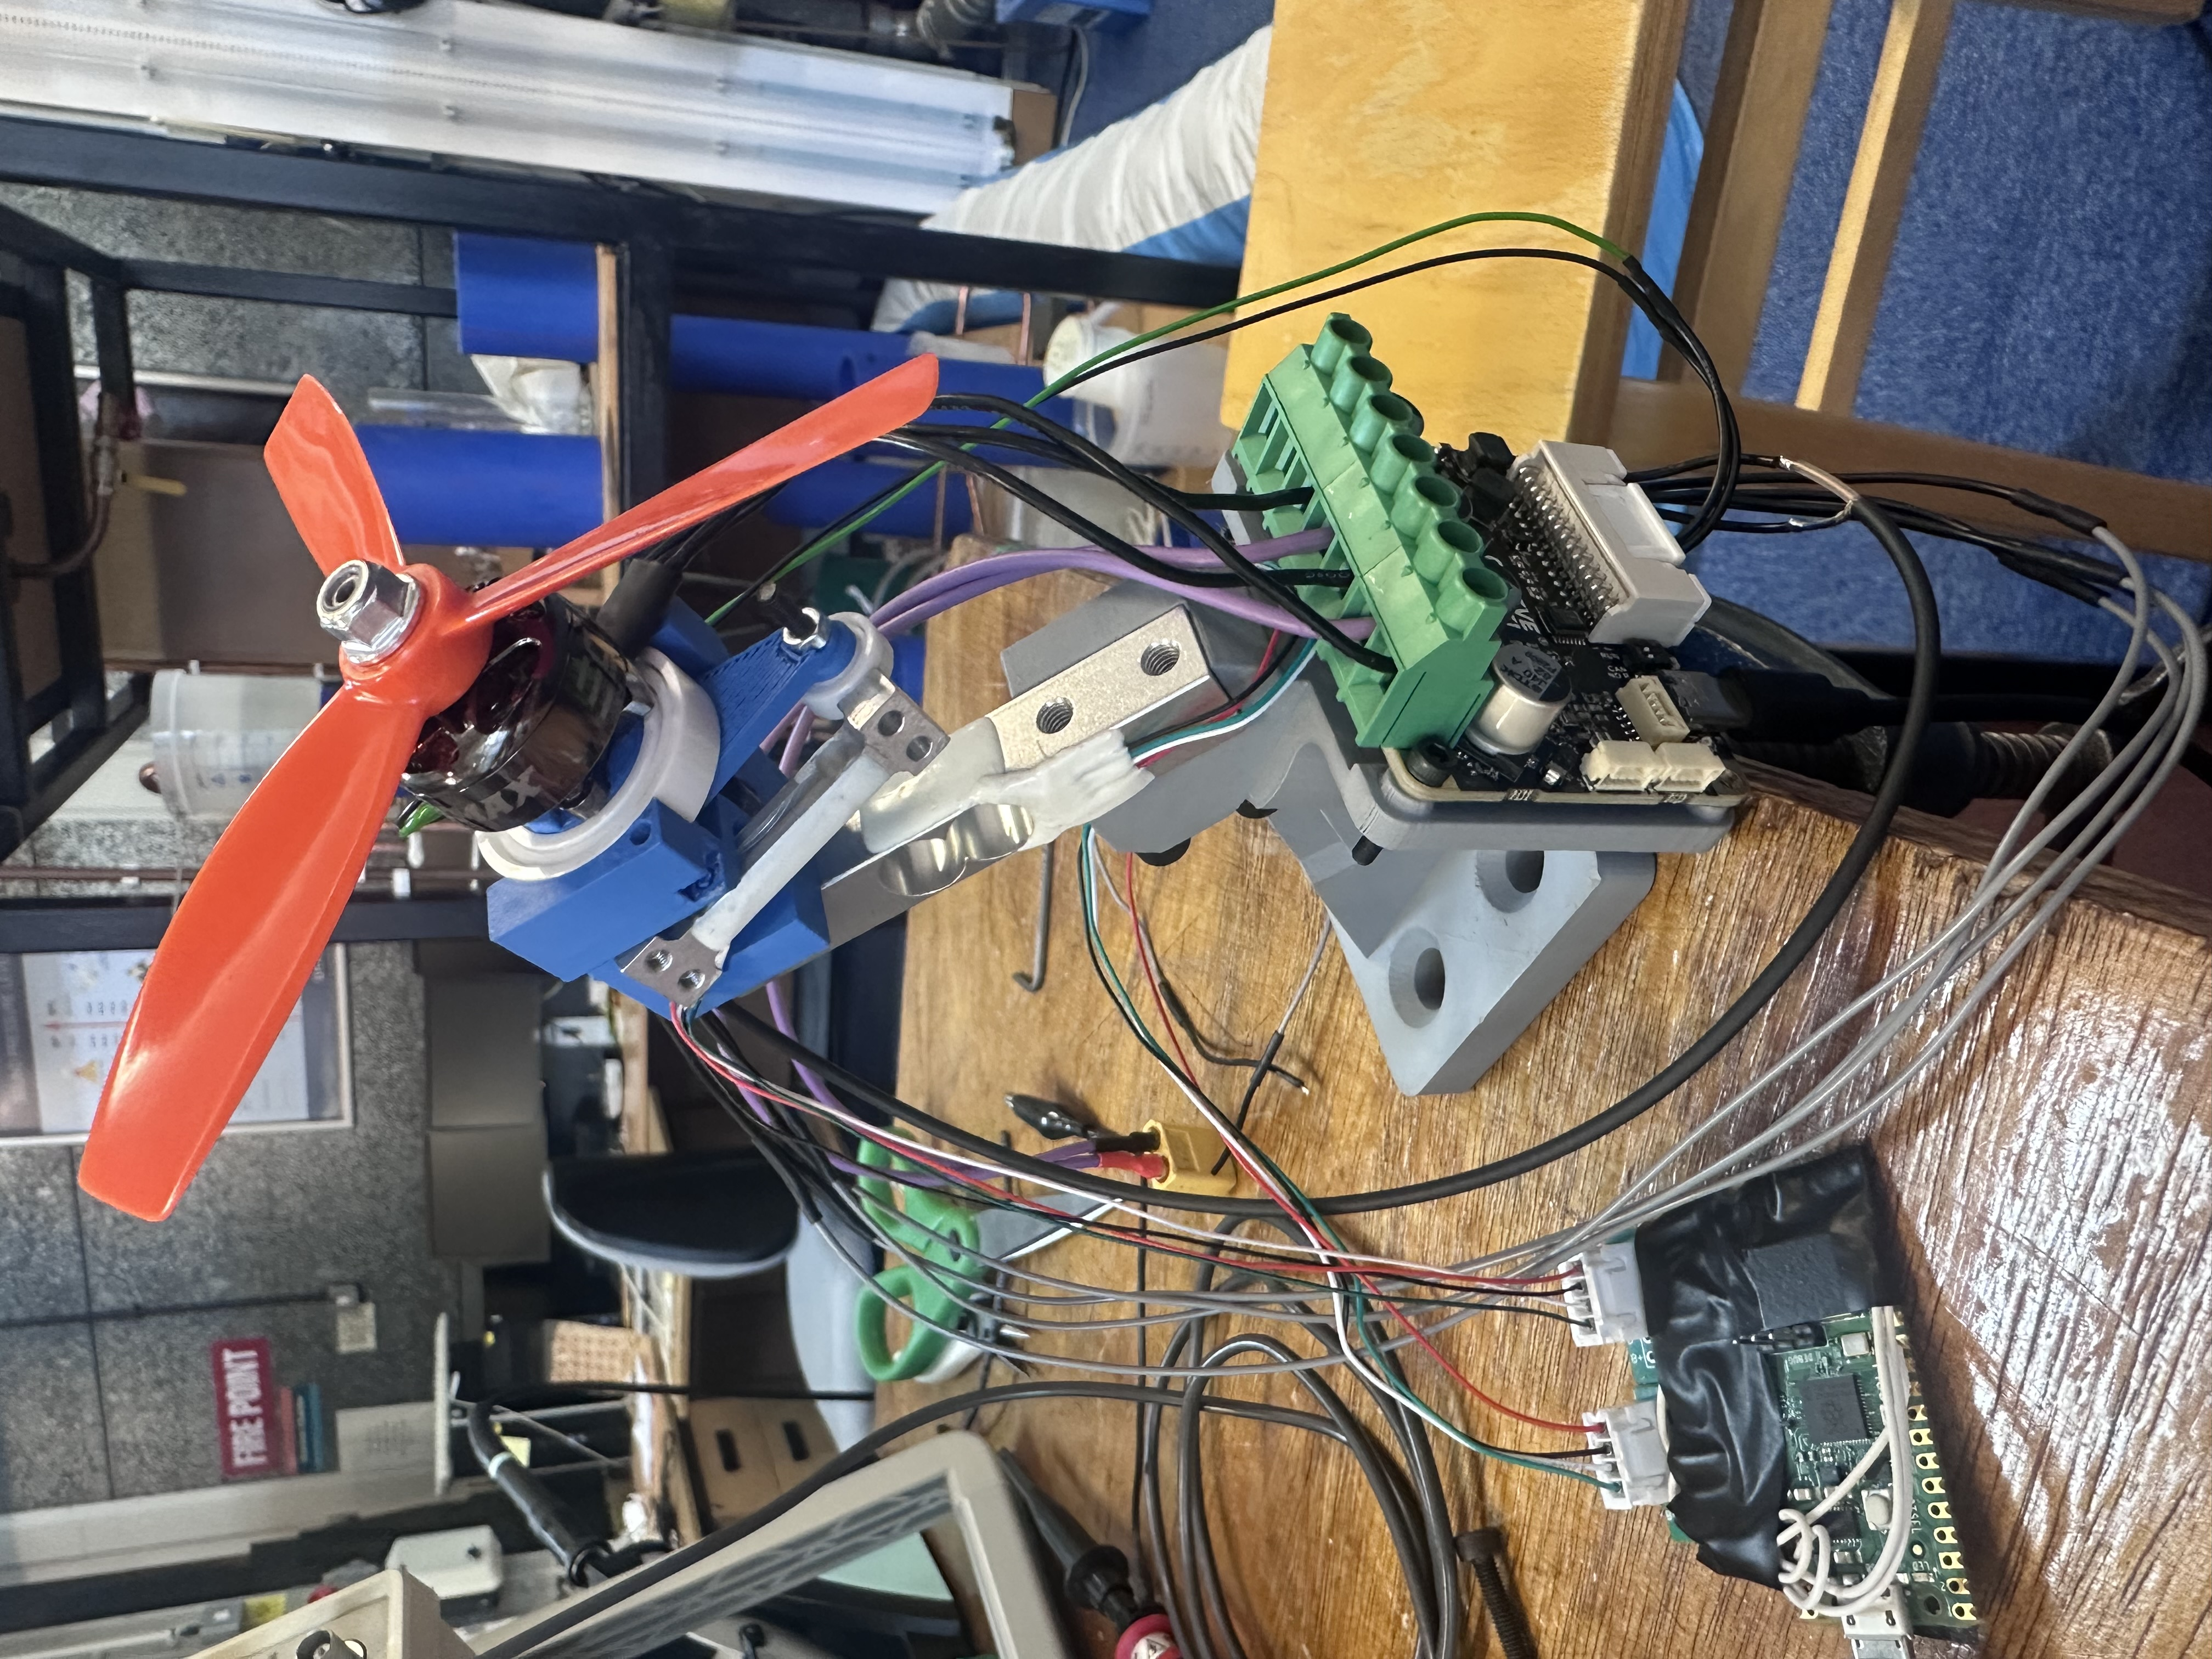
\includegraphics[height=6cm]{../final_report/figures/aero_setup.pdf}
        \end{subfigure}
    \end{figure}
\end{frame}

\begin{frame}{Acoustic setup}
    \begin{figure}
    \centering
    \begin{subfigure}{0.45\textwidth}
        \centering
        \includegraphics[height=6cm]{../final_report/tikz/mic_floor_plan.pdf}
    \end{subfigure}
    \begin{subfigure}{0.45\textwidth}
        \centering
        
\includegraphics[height=6cm]{../final_report/figures/chamber.pdf}
    \end{subfigure}
    \end{figure}
\end{frame}



\section{Results}

\begin{frame}{Aerodynamic Scaling}
    \begin{figure}
        \centering
        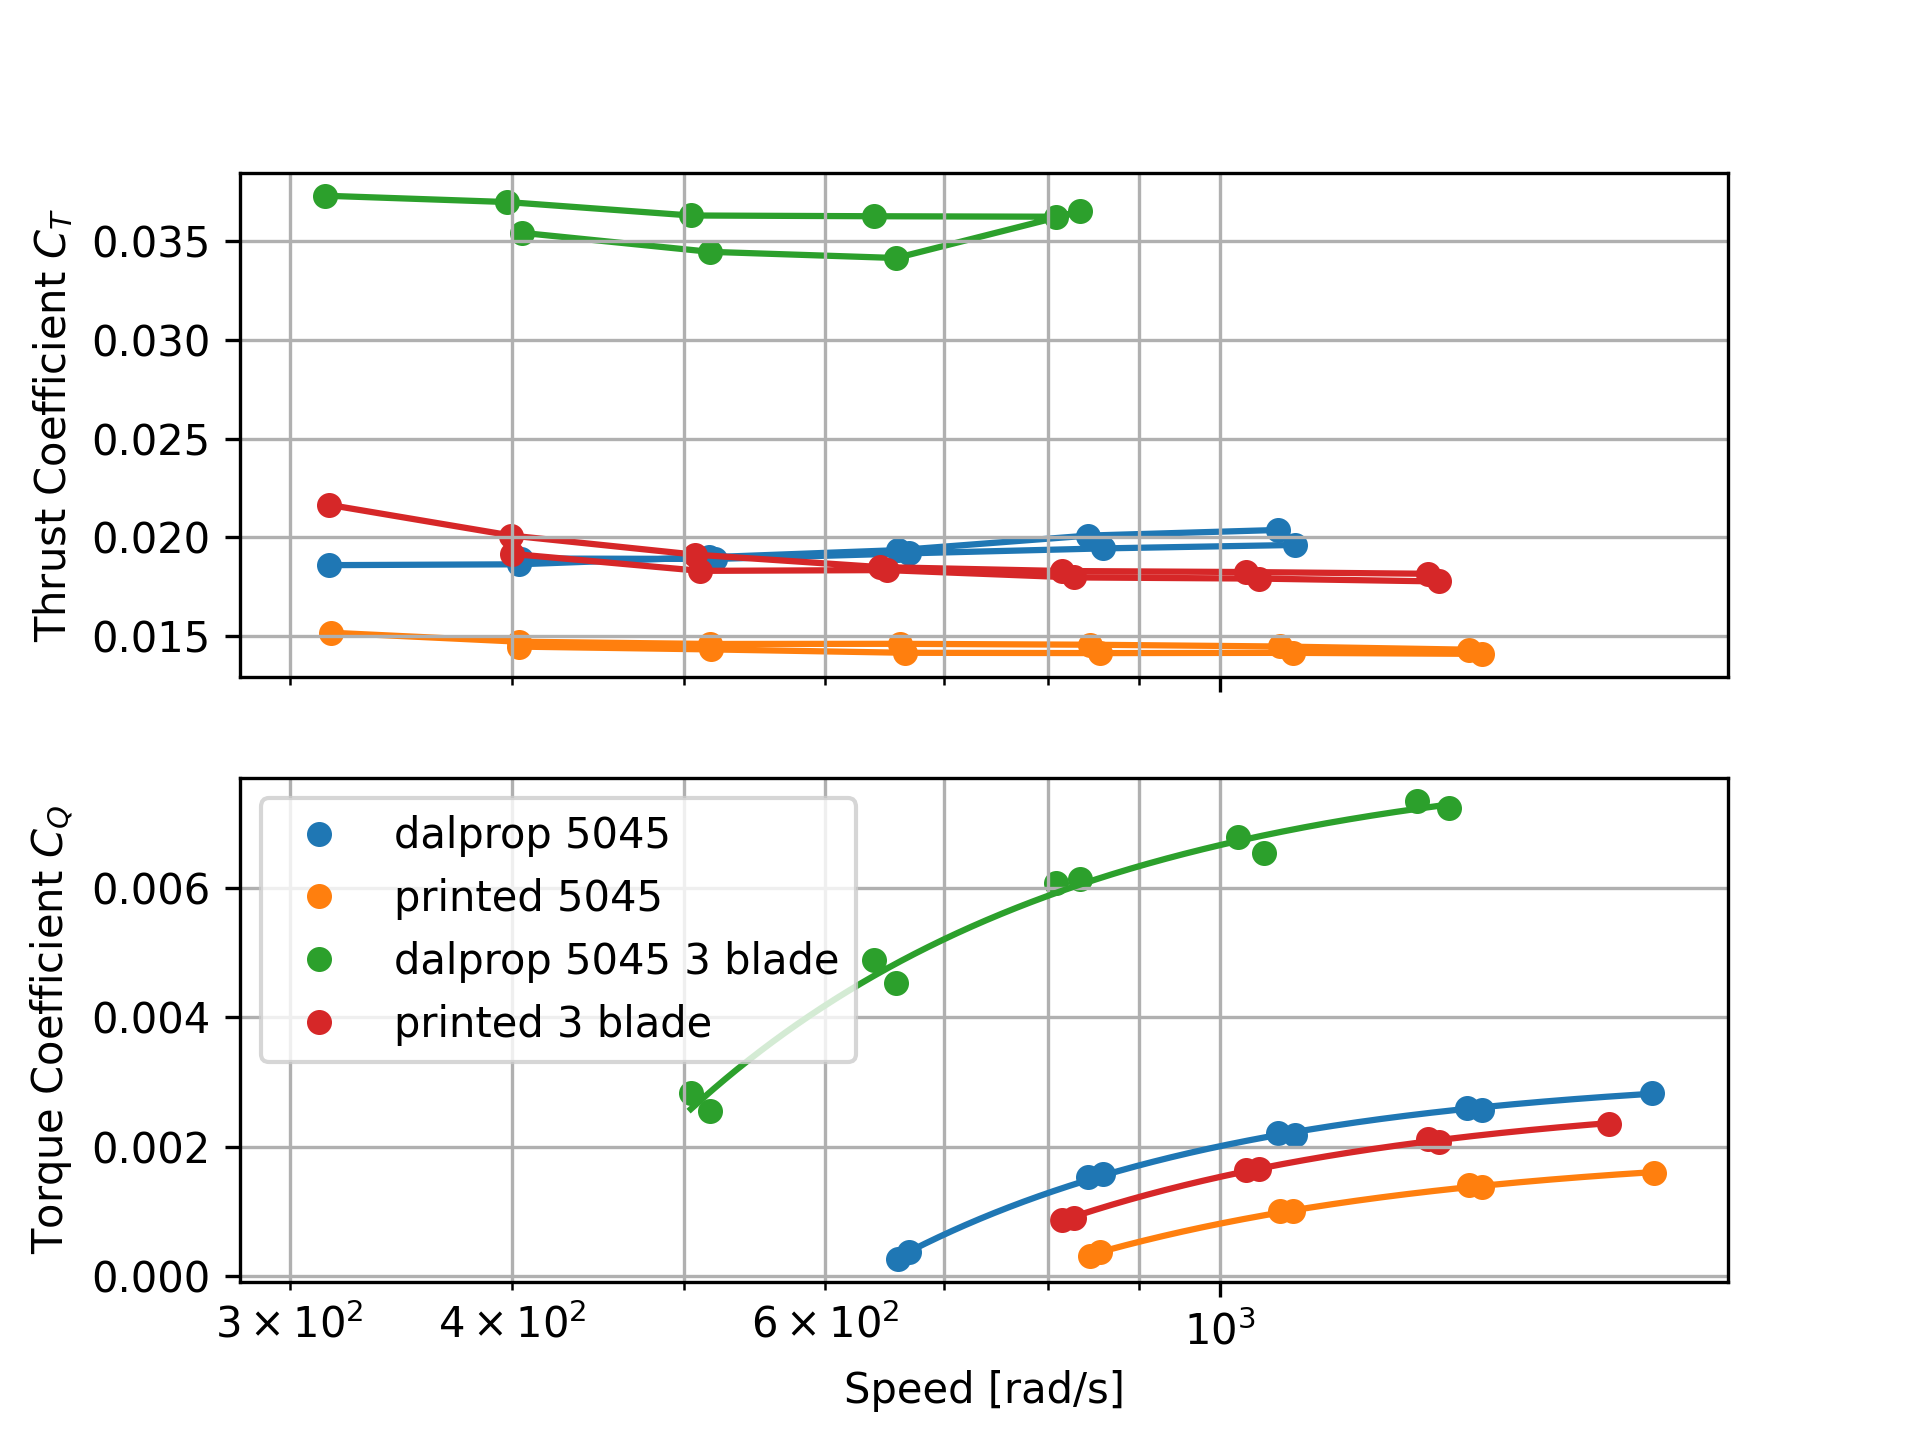
\includegraphics[width=0.8\textwidth]{../final_report/figures/printed_aero_coeffs.pdf}
    \end{figure}
\end{frame}


\begin{frame}{Acoustic Scaling}
    \begin{figure}
        \centering
        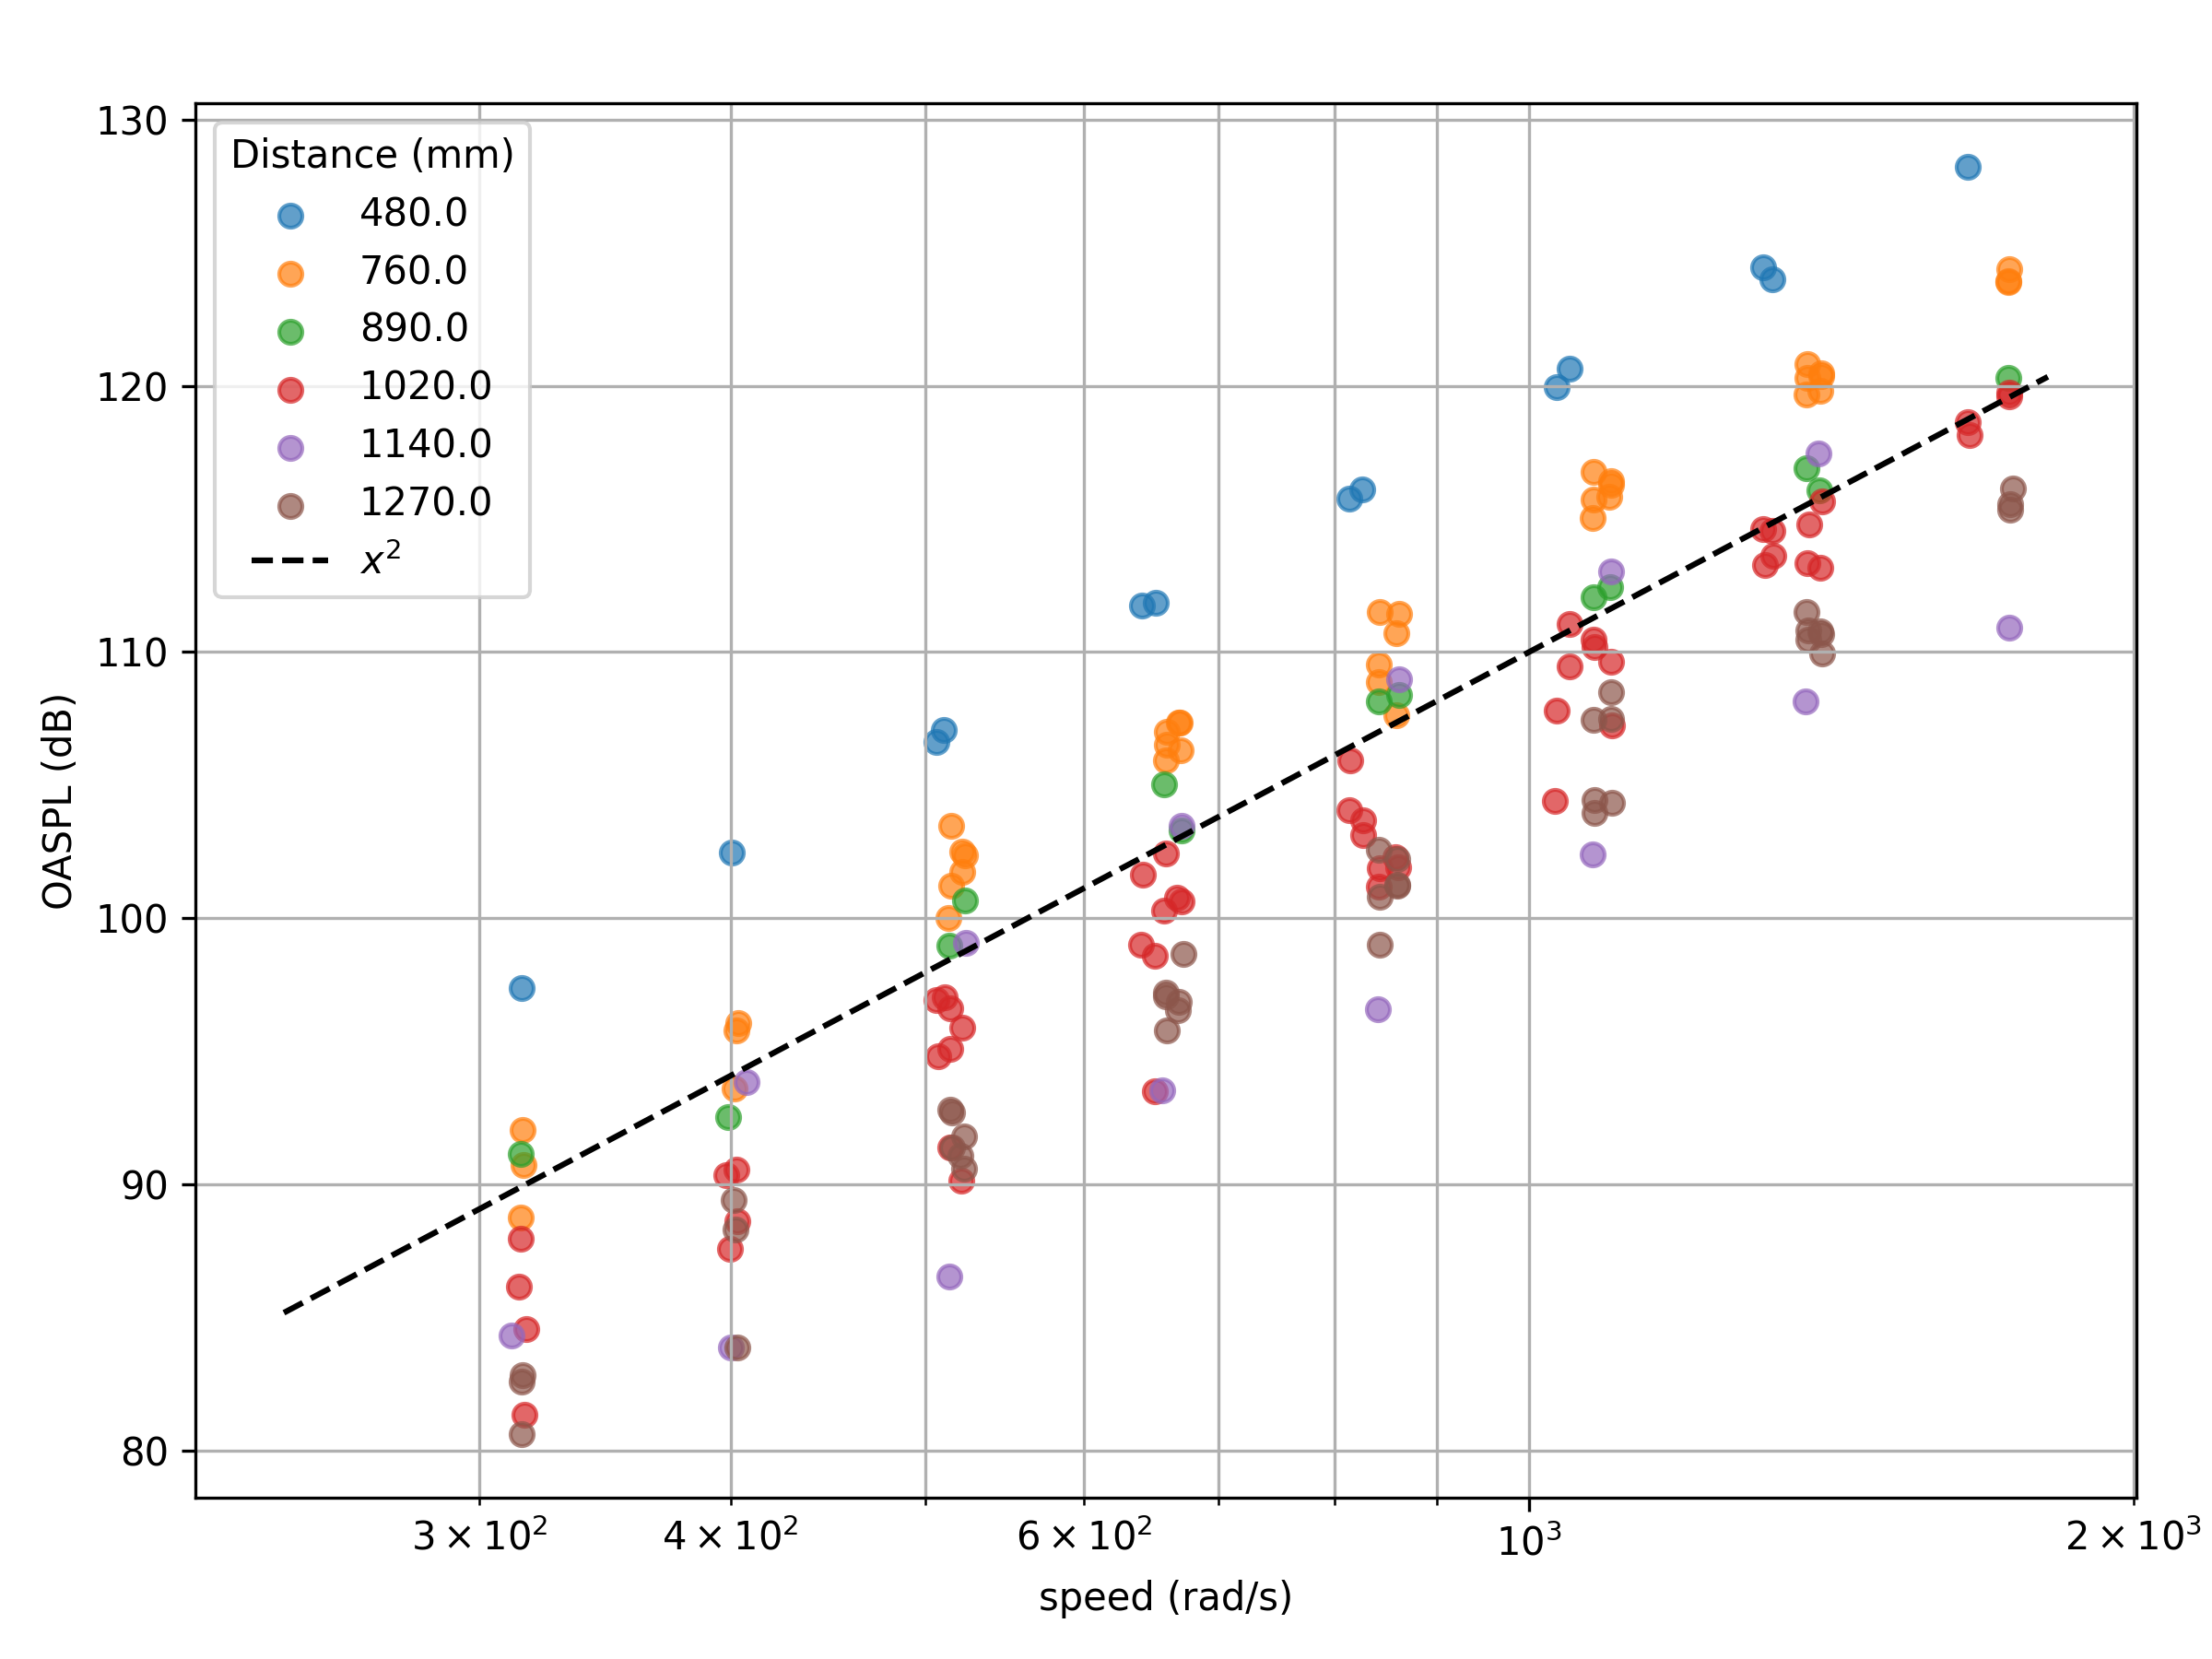
\includegraphics[width=0.8\textwidth]{../final_report/figures/spl_speed_variation.pdf}
    \end{figure}
\end{frame}

\begin{frame}{Relative Acoustic Performance}
    \begin{figure}
        \centering
        \includegraphics[width=0.8\textwidth]{../final_report/figures/OASPLref_bar.pdf}
    \end{figure}
\end{frame}

\section{Conclusion}

\begin{frame}{Conclusion}
    \begin{itemize}
        \item Small reduction in overall noise for swept and looped designs
        \vspace{1cm}
        \item Reductions in efficiency outweighed acoustic benefits.
        \vspace{1cm}
        \item Improving efficiency more effective than reducing noise.
    \end{itemize}
    \vspace{1cm}
    Questions?
\end{frame}

\begin{frame}[allowframebreaks]{References}
    \printbibliography
\end{frame}

\end{document}
